\section{Condutor esférico. Campo uniforme}

\frame{
	\frametitle{Campo elétrico de um condutor esférico}
	\begin{block}{Introdução}
		Para um corpo de pequenas dimensões e carregado de eletricidade, desprezamos o seu volume e consideramos como se fosse uma carga elétrica concentrada num ponto. Nesse caso:
		$$E = K \ \dfrac{Q}{d^2}$$ \\
		\begin{itemize}
			\item Agora iremos estudar o caso onde iremos considerar uma esfera condutora eletrizada com carga elétrica $Q$ e de raio $R$.
		\end{itemize}
	\end{block}
}

\frame{
	\frametitle{Campo elétrico de um condutor esférico}
	\begin{block}{Introdução}
		\begin{itemize}
			\item Vamos supor que essa esfera esteja em equilíbrio eletrostático e afastada de qualquer outro corpo.
			\item Como a esfera encontra-se carregada, ela produz um campo elétrico à sua volta.
			\item Sendo assim, vamos determinar o valor do campo elétrico criado por essa esfera condutora eletrizada desde pontos infinitamente afastados até pontos internos.
		\end{itemize}
	\end{block}
}

\setmyunit{1cm}

\frame{
	\frametitle{Campo elétrico de um condutor esférico}
	\begin{block}{Possibilidades}
		Um ponto pode ocupar, relativamente à esfera, três posições: ou é \textbf{interno} (ponto A), ou \textbf{pertence} à esfera (ponto B), ou é \textbf{externo} (ponto C).
	\end{block}

	\vspace{0.3cm}
	
	\centering
	\scalebox{1}{

\tikzset{every picture/.style={line width=0.75pt}} %set default line width to 0.75pt        

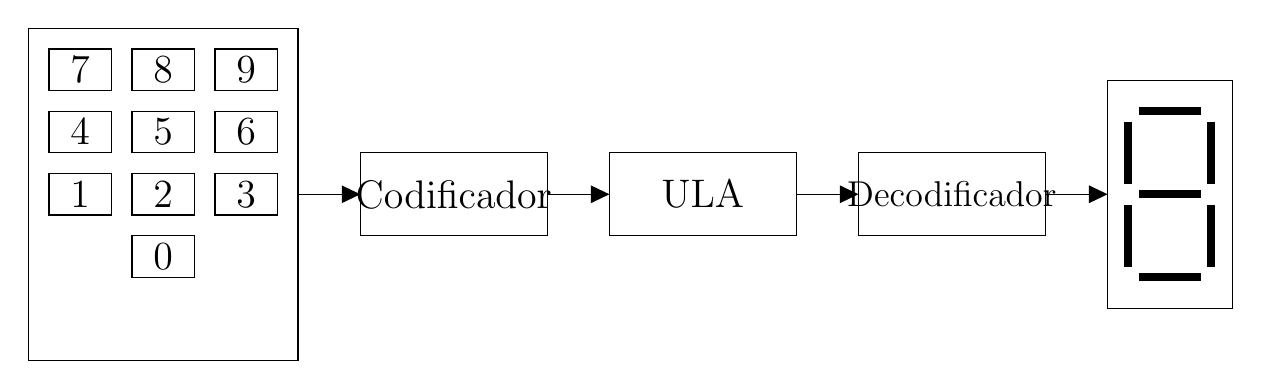
\begin{tikzpicture}[x=0.75pt,y=0.75pt,yscale=-1,xscale=1]
%uncomment if require: \path (0,300); %set diagram left start at 0, and has height of 300

%Shape: Rectangle [id:dp8798188650405219] 
\draw   (30,50) -- (160,50) -- (160,210) -- (30,210) -- cycle ;
%Shape: Rectangle [id:dp593444354888008] 
\draw   (40,60) -- (70,60) -- (70,80) -- (40,80) -- cycle ;
%Shape: Rectangle [id:dp4412846627526852] 
\draw   (80,60) -- (110,60) -- (110,80) -- (80,80) -- cycle ;
%Shape: Rectangle [id:dp2343273962035186] 
\draw   (120,60) -- (150,60) -- (150,80) -- (120,80) -- cycle ;
%Shape: Rectangle [id:dp05777918912875246] 
\draw   (40,90) -- (70,90) -- (70,110) -- (40,110) -- cycle ;
%Shape: Rectangle [id:dp9955010424516375] 
\draw   (80,90) -- (110,90) -- (110,110) -- (80,110) -- cycle ;
%Shape: Rectangle [id:dp24021539717259266] 
\draw   (120,90) -- (150,90) -- (150,110) -- (120,110) -- cycle ;
%Shape: Rectangle [id:dp36169684584711925] 
\draw   (40,120) -- (70,120) -- (70,140) -- (40,140) -- cycle ;
%Shape: Rectangle [id:dp7232437677097003] 
\draw   (80,120) -- (110,120) -- (110,140) -- (80,140) -- cycle ;
%Shape: Rectangle [id:dp6884539525496838] 
\draw   (120,120) -- (150,120) -- (150,140) -- (120,140) -- cycle ;
%Shape: Rectangle [id:dp9961423077173726] 
\draw   (80,150) -- (110,150) -- (110,170) -- (80,170) -- cycle ;
%Shape: Rectangle [id:dp6643057105712631] 
\draw   (190,110) -- (280,110) -- (280,150) -- (190,150) -- cycle ;
%Shape: Rectangle [id:dp7094011053258715] 
\draw   (550,75) -- (610,75) -- (610,185) -- (550,185) -- cycle ;
%Shape: Rectangle [id:dp2693438921699036] 
\draw   (310,110) -- (400,110) -- (400,150) -- (310,150) -- cycle ;
%Shape: Rectangle [id:dp3654960401722005] 
\draw   (430,110) -- (520,110) -- (520,150) -- (430,150) -- cycle ;
%Straight Lines [id:da6667328032348829] 
\draw    (160,130) -- (188,130) ;
\draw [shift={(190,130)}, rotate = 180] [fill={rgb, 255:red, 0; green, 0; blue, 0 }  ][line width=0.75]  [draw opacity=0] (8.93,-4.29) -- (0,0) -- (8.93,4.29) -- cycle    ;

%Straight Lines [id:da5165651690517046] 
\draw    (280,130) -- (308,130) ;
\draw [shift={(310,130)}, rotate = 180] [fill={rgb, 255:red, 0; green, 0; blue, 0 }  ][line width=0.75]  [draw opacity=0] (8.93,-4.29) -- (0,0) -- (8.93,4.29) -- cycle    ;

%Straight Lines [id:da17751850693095572] 
\draw    (400,130) -- (428,130) ;
\draw [shift={(430,130)}, rotate = 180] [fill={rgb, 255:red, 0; green, 0; blue, 0 }  ][line width=0.75]  [draw opacity=0] (8.93,-4.29) -- (0,0) -- (8.93,4.29) -- cycle    ;

%Straight Lines [id:da4998570413390182] 
\draw [color={rgb, 255:red, 0; green, 0; blue, 0 }  ,draw opacity=1 ][line width=3]    (560,95) -- (560,125) ;


%Straight Lines [id:da05287212083080073] 
\draw [color={rgb, 255:red, 0; green, 0; blue, 0 }  ,draw opacity=1 ][line width=3]    (600,95) -- (600,125) ;


%Straight Lines [id:da9146969001147236] 
\draw [color={rgb, 255:red, 0; green, 0; blue, 0 }  ,draw opacity=1 ][line width=3]    (560,135) -- (560,165) ;


%Straight Lines [id:da37610179690179124] 
\draw [color={rgb, 255:red, 0; green, 0; blue, 0 }  ,draw opacity=1 ][line width=3]    (600,135) -- (600,165) ;


%Straight Lines [id:da2798262228013664] 
\draw [color={rgb, 255:red, 0; green, 0; blue, 0 }  ,draw opacity=1 ][line width=3]    (595,130) -- (565,130) ;


%Straight Lines [id:da15184615547446478] 
\draw [color={rgb, 255:red, 0; green, 0; blue, 0 }  ,draw opacity=1 ][line width=3]    (595,90) -- (565,90) ;


%Straight Lines [id:da20609816632014244] 
\draw [color={rgb, 255:red, 0; green, 0; blue, 0 }  ,draw opacity=1 ][line width=3]    (595,170) -- (565,170) ;


%Straight Lines [id:da16937059284664002] 
\draw    (520,130) -- (548,130) ;
\draw [shift={(550,130)}, rotate = 180] [fill={rgb, 255:red, 0; green, 0; blue, 0 }  ][line width=0.75]  [draw opacity=0] (8.93,-4.29) -- (0,0) -- (8.93,4.29) -- cycle    ;


% Text Node
\draw (135,70) node   {\Large $9$};
% Text Node
\draw (95,70) node   {\Large $8$};
% Text Node
\draw (55,70) node   {\Large $7$};
% Text Node
\draw (135,100) node   {\Large $6$};
% Text Node
\draw (135,130) node   {\Large $3$};
% Text Node
\draw (95,160) node   {\Large $0$};
% Text Node
\draw (95,130) node   {\Large $2$};
% Text Node
\draw (95,100) node   {\Large $5$};
% Text Node
\draw (55,100) node   {\Large $4$};
% Text Node
\draw (55,130) node   {\Large $1$};
% Text Node
\draw (235,130) node  [align=left] {\Large Codificador};
% Text Node
\draw (355,130) node  [align=left] {\Large ULA};
% Text Node
\draw (475,130) node [scale=0.9] [align=left] {\Large Decodificador};


\end{tikzpicture}
}
%	\centerline{\includegraphics[width=0.45\linewidth]{Figuras/Ch08/condutor.png}}
}

\frame{
	\frametitle{Campo elétrico de um condutor esférico}
	\begin{block}{Caso $\#$01: ponto $A$ interno}
		A intensidade do vetor campo elétrico no interior de um condutor carregado de eletricidade e em equilíbrio eletrostático é sempre \textbf{nulo}.
	\end{block}
	
	\vspace{0.3cm}
	
	\centering
	\scalebox{1}{

\tikzset{every picture/.style={line width=0.75pt}} %set default line width to 0.75pt        

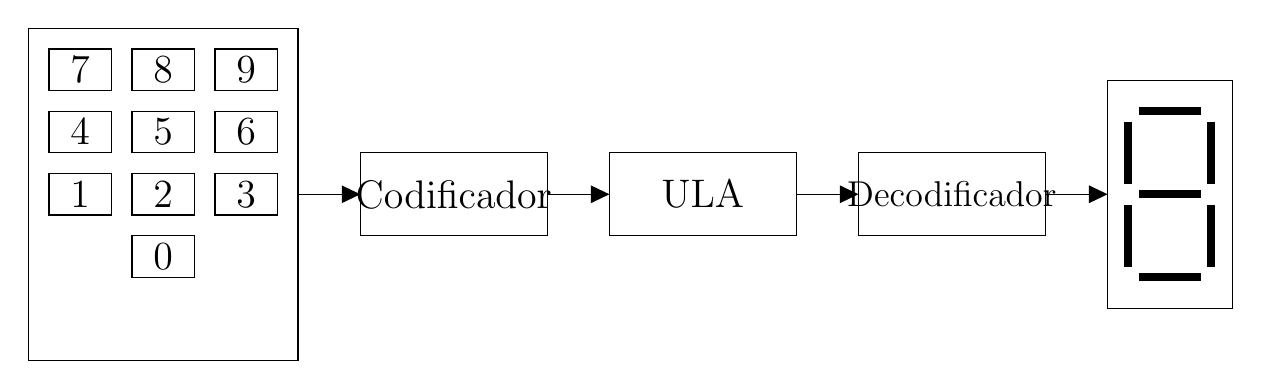
\begin{tikzpicture}[x=0.75pt,y=0.75pt,yscale=-1,xscale=1]
%uncomment if require: \path (0,300); %set diagram left start at 0, and has height of 300

%Shape: Rectangle [id:dp8798188650405219] 
\draw   (30,50) -- (160,50) -- (160,210) -- (30,210) -- cycle ;
%Shape: Rectangle [id:dp593444354888008] 
\draw   (40,60) -- (70,60) -- (70,80) -- (40,80) -- cycle ;
%Shape: Rectangle [id:dp4412846627526852] 
\draw   (80,60) -- (110,60) -- (110,80) -- (80,80) -- cycle ;
%Shape: Rectangle [id:dp2343273962035186] 
\draw   (120,60) -- (150,60) -- (150,80) -- (120,80) -- cycle ;
%Shape: Rectangle [id:dp05777918912875246] 
\draw   (40,90) -- (70,90) -- (70,110) -- (40,110) -- cycle ;
%Shape: Rectangle [id:dp9955010424516375] 
\draw   (80,90) -- (110,90) -- (110,110) -- (80,110) -- cycle ;
%Shape: Rectangle [id:dp24021539717259266] 
\draw   (120,90) -- (150,90) -- (150,110) -- (120,110) -- cycle ;
%Shape: Rectangle [id:dp36169684584711925] 
\draw   (40,120) -- (70,120) -- (70,140) -- (40,140) -- cycle ;
%Shape: Rectangle [id:dp7232437677097003] 
\draw   (80,120) -- (110,120) -- (110,140) -- (80,140) -- cycle ;
%Shape: Rectangle [id:dp6884539525496838] 
\draw   (120,120) -- (150,120) -- (150,140) -- (120,140) -- cycle ;
%Shape: Rectangle [id:dp9961423077173726] 
\draw   (80,150) -- (110,150) -- (110,170) -- (80,170) -- cycle ;
%Shape: Rectangle [id:dp6643057105712631] 
\draw   (190,110) -- (280,110) -- (280,150) -- (190,150) -- cycle ;
%Shape: Rectangle [id:dp7094011053258715] 
\draw   (550,75) -- (610,75) -- (610,185) -- (550,185) -- cycle ;
%Shape: Rectangle [id:dp2693438921699036] 
\draw   (310,110) -- (400,110) -- (400,150) -- (310,150) -- cycle ;
%Shape: Rectangle [id:dp3654960401722005] 
\draw   (430,110) -- (520,110) -- (520,150) -- (430,150) -- cycle ;
%Straight Lines [id:da6667328032348829] 
\draw    (160,130) -- (188,130) ;
\draw [shift={(190,130)}, rotate = 180] [fill={rgb, 255:red, 0; green, 0; blue, 0 }  ][line width=0.75]  [draw opacity=0] (8.93,-4.29) -- (0,0) -- (8.93,4.29) -- cycle    ;

%Straight Lines [id:da5165651690517046] 
\draw    (280,130) -- (308,130) ;
\draw [shift={(310,130)}, rotate = 180] [fill={rgb, 255:red, 0; green, 0; blue, 0 }  ][line width=0.75]  [draw opacity=0] (8.93,-4.29) -- (0,0) -- (8.93,4.29) -- cycle    ;

%Straight Lines [id:da17751850693095572] 
\draw    (400,130) -- (428,130) ;
\draw [shift={(430,130)}, rotate = 180] [fill={rgb, 255:red, 0; green, 0; blue, 0 }  ][line width=0.75]  [draw opacity=0] (8.93,-4.29) -- (0,0) -- (8.93,4.29) -- cycle    ;

%Straight Lines [id:da4998570413390182] 
\draw [color={rgb, 255:red, 0; green, 0; blue, 0 }  ,draw opacity=1 ][line width=3]    (560,95) -- (560,125) ;


%Straight Lines [id:da05287212083080073] 
\draw [color={rgb, 255:red, 0; green, 0; blue, 0 }  ,draw opacity=1 ][line width=3]    (600,95) -- (600,125) ;


%Straight Lines [id:da9146969001147236] 
\draw [color={rgb, 255:red, 0; green, 0; blue, 0 }  ,draw opacity=1 ][line width=3]    (560,135) -- (560,165) ;


%Straight Lines [id:da37610179690179124] 
\draw [color={rgb, 255:red, 0; green, 0; blue, 0 }  ,draw opacity=1 ][line width=3]    (600,135) -- (600,165) ;


%Straight Lines [id:da2798262228013664] 
\draw [color={rgb, 255:red, 0; green, 0; blue, 0 }  ,draw opacity=1 ][line width=3]    (595,130) -- (565,130) ;


%Straight Lines [id:da15184615547446478] 
\draw [color={rgb, 255:red, 0; green, 0; blue, 0 }  ,draw opacity=1 ][line width=3]    (595,90) -- (565,90) ;


%Straight Lines [id:da20609816632014244] 
\draw [color={rgb, 255:red, 0; green, 0; blue, 0 }  ,draw opacity=1 ][line width=3]    (595,170) -- (565,170) ;


%Straight Lines [id:da16937059284664002] 
\draw    (520,130) -- (548,130) ;
\draw [shift={(550,130)}, rotate = 180] [fill={rgb, 255:red, 0; green, 0; blue, 0 }  ][line width=0.75]  [draw opacity=0] (8.93,-4.29) -- (0,0) -- (8.93,4.29) -- cycle    ;


% Text Node
\draw (135,70) node   {\Large $9$};
% Text Node
\draw (95,70) node   {\Large $8$};
% Text Node
\draw (55,70) node   {\Large $7$};
% Text Node
\draw (135,100) node   {\Large $6$};
% Text Node
\draw (135,130) node   {\Large $3$};
% Text Node
\draw (95,160) node   {\Large $0$};
% Text Node
\draw (95,130) node   {\Large $2$};
% Text Node
\draw (95,100) node   {\Large $5$};
% Text Node
\draw (55,100) node   {\Large $4$};
% Text Node
\draw (55,130) node   {\Large $1$};
% Text Node
\draw (235,130) node  [align=left] {\Large Codificador};
% Text Node
\draw (355,130) node  [align=left] {\Large ULA};
% Text Node
\draw (475,130) node [scale=0.9] [align=left] {\Large Decodificador};


\end{tikzpicture}
}
%	\centerline{\includegraphics[width=0.45\linewidth]{Figuras/Ch08/condutor.png}}
}

\frame{
	\frametitle{Campo elétrico de um condutor esférico}
	\begin{block}{Caso $\#$02: ponto $B$ pertencente à esfera}
		Dependendo do modelo adotado para a distribuição de carga a resposta é diferente. Em livros razoáveis de ensino médio e mesmo em livros de Física Geral de ensino superior o assunto é convenientemente evitado pelos autores.
		\begin{itemize}
			\item Este tema não é adequado ao ensino médio.
		\end{itemize}
	\end{block}

%	\vspace{0.3cm}
	
	\centering
	\scalebox{1}{

\tikzset{every picture/.style={line width=0.75pt}} %set default line width to 0.75pt        

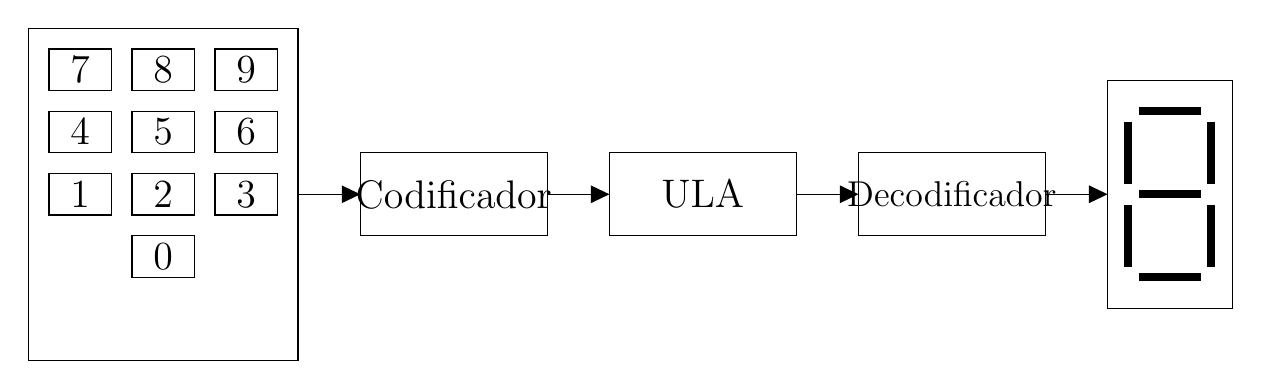
\begin{tikzpicture}[x=0.75pt,y=0.75pt,yscale=-1,xscale=1]
%uncomment if require: \path (0,300); %set diagram left start at 0, and has height of 300

%Shape: Rectangle [id:dp8798188650405219] 
\draw   (30,50) -- (160,50) -- (160,210) -- (30,210) -- cycle ;
%Shape: Rectangle [id:dp593444354888008] 
\draw   (40,60) -- (70,60) -- (70,80) -- (40,80) -- cycle ;
%Shape: Rectangle [id:dp4412846627526852] 
\draw   (80,60) -- (110,60) -- (110,80) -- (80,80) -- cycle ;
%Shape: Rectangle [id:dp2343273962035186] 
\draw   (120,60) -- (150,60) -- (150,80) -- (120,80) -- cycle ;
%Shape: Rectangle [id:dp05777918912875246] 
\draw   (40,90) -- (70,90) -- (70,110) -- (40,110) -- cycle ;
%Shape: Rectangle [id:dp9955010424516375] 
\draw   (80,90) -- (110,90) -- (110,110) -- (80,110) -- cycle ;
%Shape: Rectangle [id:dp24021539717259266] 
\draw   (120,90) -- (150,90) -- (150,110) -- (120,110) -- cycle ;
%Shape: Rectangle [id:dp36169684584711925] 
\draw   (40,120) -- (70,120) -- (70,140) -- (40,140) -- cycle ;
%Shape: Rectangle [id:dp7232437677097003] 
\draw   (80,120) -- (110,120) -- (110,140) -- (80,140) -- cycle ;
%Shape: Rectangle [id:dp6884539525496838] 
\draw   (120,120) -- (150,120) -- (150,140) -- (120,140) -- cycle ;
%Shape: Rectangle [id:dp9961423077173726] 
\draw   (80,150) -- (110,150) -- (110,170) -- (80,170) -- cycle ;
%Shape: Rectangle [id:dp6643057105712631] 
\draw   (190,110) -- (280,110) -- (280,150) -- (190,150) -- cycle ;
%Shape: Rectangle [id:dp7094011053258715] 
\draw   (550,75) -- (610,75) -- (610,185) -- (550,185) -- cycle ;
%Shape: Rectangle [id:dp2693438921699036] 
\draw   (310,110) -- (400,110) -- (400,150) -- (310,150) -- cycle ;
%Shape: Rectangle [id:dp3654960401722005] 
\draw   (430,110) -- (520,110) -- (520,150) -- (430,150) -- cycle ;
%Straight Lines [id:da6667328032348829] 
\draw    (160,130) -- (188,130) ;
\draw [shift={(190,130)}, rotate = 180] [fill={rgb, 255:red, 0; green, 0; blue, 0 }  ][line width=0.75]  [draw opacity=0] (8.93,-4.29) -- (0,0) -- (8.93,4.29) -- cycle    ;

%Straight Lines [id:da5165651690517046] 
\draw    (280,130) -- (308,130) ;
\draw [shift={(310,130)}, rotate = 180] [fill={rgb, 255:red, 0; green, 0; blue, 0 }  ][line width=0.75]  [draw opacity=0] (8.93,-4.29) -- (0,0) -- (8.93,4.29) -- cycle    ;

%Straight Lines [id:da17751850693095572] 
\draw    (400,130) -- (428,130) ;
\draw [shift={(430,130)}, rotate = 180] [fill={rgb, 255:red, 0; green, 0; blue, 0 }  ][line width=0.75]  [draw opacity=0] (8.93,-4.29) -- (0,0) -- (8.93,4.29) -- cycle    ;

%Straight Lines [id:da4998570413390182] 
\draw [color={rgb, 255:red, 0; green, 0; blue, 0 }  ,draw opacity=1 ][line width=3]    (560,95) -- (560,125) ;


%Straight Lines [id:da05287212083080073] 
\draw [color={rgb, 255:red, 0; green, 0; blue, 0 }  ,draw opacity=1 ][line width=3]    (600,95) -- (600,125) ;


%Straight Lines [id:da9146969001147236] 
\draw [color={rgb, 255:red, 0; green, 0; blue, 0 }  ,draw opacity=1 ][line width=3]    (560,135) -- (560,165) ;


%Straight Lines [id:da37610179690179124] 
\draw [color={rgb, 255:red, 0; green, 0; blue, 0 }  ,draw opacity=1 ][line width=3]    (600,135) -- (600,165) ;


%Straight Lines [id:da2798262228013664] 
\draw [color={rgb, 255:red, 0; green, 0; blue, 0 }  ,draw opacity=1 ][line width=3]    (595,130) -- (565,130) ;


%Straight Lines [id:da15184615547446478] 
\draw [color={rgb, 255:red, 0; green, 0; blue, 0 }  ,draw opacity=1 ][line width=3]    (595,90) -- (565,90) ;


%Straight Lines [id:da20609816632014244] 
\draw [color={rgb, 255:red, 0; green, 0; blue, 0 }  ,draw opacity=1 ][line width=3]    (595,170) -- (565,170) ;


%Straight Lines [id:da16937059284664002] 
\draw    (520,130) -- (548,130) ;
\draw [shift={(550,130)}, rotate = 180] [fill={rgb, 255:red, 0; green, 0; blue, 0 }  ][line width=0.75]  [draw opacity=0] (8.93,-4.29) -- (0,0) -- (8.93,4.29) -- cycle    ;


% Text Node
\draw (135,70) node   {\Large $9$};
% Text Node
\draw (95,70) node   {\Large $8$};
% Text Node
\draw (55,70) node   {\Large $7$};
% Text Node
\draw (135,100) node   {\Large $6$};
% Text Node
\draw (135,130) node   {\Large $3$};
% Text Node
\draw (95,160) node   {\Large $0$};
% Text Node
\draw (95,130) node   {\Large $2$};
% Text Node
\draw (95,100) node   {\Large $5$};
% Text Node
\draw (55,100) node   {\Large $4$};
% Text Node
\draw (55,130) node   {\Large $1$};
% Text Node
\draw (235,130) node  [align=left] {\Large Codificador};
% Text Node
\draw (355,130) node  [align=left] {\Large ULA};
% Text Node
\draw (475,130) node [scale=0.9] [align=left] {\Large Decodificador};


\end{tikzpicture}
}
}

\frame{
	\frametitle{Campo elétrico de um condutor esférico}
	\begin{block}{Caso $\#$03: ponto $C$ externo}
		O campo produzido num ponto externo de uma esfera pode ser calculado admitindo-se que a carga da esfera seja \textbf{puntiforme} e colocada no \textbf{centro da esfera}, em vez de estar distribuída pela superfície.
		$$E = K \ \dfrac{Q}{d^2}$$
	\end{block}
	
%	\vspace{0.3cm}
	
	\centering
	\scalebox{1}{

\tikzset{every picture/.style={line width=0.75pt}} %set default line width to 0.75pt        

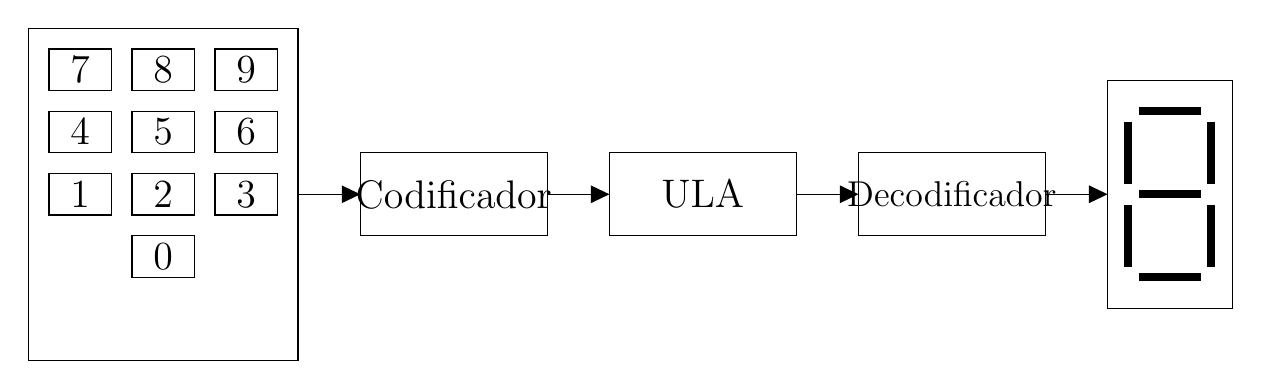
\begin{tikzpicture}[x=0.75pt,y=0.75pt,yscale=-1,xscale=1]
%uncomment if require: \path (0,300); %set diagram left start at 0, and has height of 300

%Shape: Rectangle [id:dp8798188650405219] 
\draw   (30,50) -- (160,50) -- (160,210) -- (30,210) -- cycle ;
%Shape: Rectangle [id:dp593444354888008] 
\draw   (40,60) -- (70,60) -- (70,80) -- (40,80) -- cycle ;
%Shape: Rectangle [id:dp4412846627526852] 
\draw   (80,60) -- (110,60) -- (110,80) -- (80,80) -- cycle ;
%Shape: Rectangle [id:dp2343273962035186] 
\draw   (120,60) -- (150,60) -- (150,80) -- (120,80) -- cycle ;
%Shape: Rectangle [id:dp05777918912875246] 
\draw   (40,90) -- (70,90) -- (70,110) -- (40,110) -- cycle ;
%Shape: Rectangle [id:dp9955010424516375] 
\draw   (80,90) -- (110,90) -- (110,110) -- (80,110) -- cycle ;
%Shape: Rectangle [id:dp24021539717259266] 
\draw   (120,90) -- (150,90) -- (150,110) -- (120,110) -- cycle ;
%Shape: Rectangle [id:dp36169684584711925] 
\draw   (40,120) -- (70,120) -- (70,140) -- (40,140) -- cycle ;
%Shape: Rectangle [id:dp7232437677097003] 
\draw   (80,120) -- (110,120) -- (110,140) -- (80,140) -- cycle ;
%Shape: Rectangle [id:dp6884539525496838] 
\draw   (120,120) -- (150,120) -- (150,140) -- (120,140) -- cycle ;
%Shape: Rectangle [id:dp9961423077173726] 
\draw   (80,150) -- (110,150) -- (110,170) -- (80,170) -- cycle ;
%Shape: Rectangle [id:dp6643057105712631] 
\draw   (190,110) -- (280,110) -- (280,150) -- (190,150) -- cycle ;
%Shape: Rectangle [id:dp7094011053258715] 
\draw   (550,75) -- (610,75) -- (610,185) -- (550,185) -- cycle ;
%Shape: Rectangle [id:dp2693438921699036] 
\draw   (310,110) -- (400,110) -- (400,150) -- (310,150) -- cycle ;
%Shape: Rectangle [id:dp3654960401722005] 
\draw   (430,110) -- (520,110) -- (520,150) -- (430,150) -- cycle ;
%Straight Lines [id:da6667328032348829] 
\draw    (160,130) -- (188,130) ;
\draw [shift={(190,130)}, rotate = 180] [fill={rgb, 255:red, 0; green, 0; blue, 0 }  ][line width=0.75]  [draw opacity=0] (8.93,-4.29) -- (0,0) -- (8.93,4.29) -- cycle    ;

%Straight Lines [id:da5165651690517046] 
\draw    (280,130) -- (308,130) ;
\draw [shift={(310,130)}, rotate = 180] [fill={rgb, 255:red, 0; green, 0; blue, 0 }  ][line width=0.75]  [draw opacity=0] (8.93,-4.29) -- (0,0) -- (8.93,4.29) -- cycle    ;

%Straight Lines [id:da17751850693095572] 
\draw    (400,130) -- (428,130) ;
\draw [shift={(430,130)}, rotate = 180] [fill={rgb, 255:red, 0; green, 0; blue, 0 }  ][line width=0.75]  [draw opacity=0] (8.93,-4.29) -- (0,0) -- (8.93,4.29) -- cycle    ;

%Straight Lines [id:da4998570413390182] 
\draw [color={rgb, 255:red, 0; green, 0; blue, 0 }  ,draw opacity=1 ][line width=3]    (560,95) -- (560,125) ;


%Straight Lines [id:da05287212083080073] 
\draw [color={rgb, 255:red, 0; green, 0; blue, 0 }  ,draw opacity=1 ][line width=3]    (600,95) -- (600,125) ;


%Straight Lines [id:da9146969001147236] 
\draw [color={rgb, 255:red, 0; green, 0; blue, 0 }  ,draw opacity=1 ][line width=3]    (560,135) -- (560,165) ;


%Straight Lines [id:da37610179690179124] 
\draw [color={rgb, 255:red, 0; green, 0; blue, 0 }  ,draw opacity=1 ][line width=3]    (600,135) -- (600,165) ;


%Straight Lines [id:da2798262228013664] 
\draw [color={rgb, 255:red, 0; green, 0; blue, 0 }  ,draw opacity=1 ][line width=3]    (595,130) -- (565,130) ;


%Straight Lines [id:da15184615547446478] 
\draw [color={rgb, 255:red, 0; green, 0; blue, 0 }  ,draw opacity=1 ][line width=3]    (595,90) -- (565,90) ;


%Straight Lines [id:da20609816632014244] 
\draw [color={rgb, 255:red, 0; green, 0; blue, 0 }  ,draw opacity=1 ][line width=3]    (595,170) -- (565,170) ;


%Straight Lines [id:da16937059284664002] 
\draw    (520,130) -- (548,130) ;
\draw [shift={(550,130)}, rotate = 180] [fill={rgb, 255:red, 0; green, 0; blue, 0 }  ][line width=0.75]  [draw opacity=0] (8.93,-4.29) -- (0,0) -- (8.93,4.29) -- cycle    ;


% Text Node
\draw (135,70) node   {\Large $9$};
% Text Node
\draw (95,70) node   {\Large $8$};
% Text Node
\draw (55,70) node   {\Large $7$};
% Text Node
\draw (135,100) node   {\Large $6$};
% Text Node
\draw (135,130) node   {\Large $3$};
% Text Node
\draw (95,160) node   {\Large $0$};
% Text Node
\draw (95,130) node   {\Large $2$};
% Text Node
\draw (95,100) node   {\Large $5$};
% Text Node
\draw (55,100) node   {\Large $4$};
% Text Node
\draw (55,130) node   {\Large $1$};
% Text Node
\draw (235,130) node  [align=left] {\Large Codificador};
% Text Node
\draw (355,130) node  [align=left] {\Large ULA};
% Text Node
\draw (475,130) node [scale=0.9] [align=left] {\Large Decodificador};


\end{tikzpicture}
}
}

\frame{
	\frametitle{Campo elétrico de um condutor esférico}
	\begin{block}{Exemplo \#01}
		Uma esfera condutora de raio $R = \SI{40}{\centi\meter}$ está eletrizada uniformemente com carga $Q = \SI{4.0}{\micro\coulomb}$. (a) Determine a intensidade do campo elétrico num ponto $P$ à \SI{60}{\centi\meter} da superfície da esfera. (b) Qual o valor da força sobre uma carga de prova $q = \SI{2.0}{\micro\coulomb}$ colocada no ponto $P$?
	\end{block}
}

\frame{
	\frametitle{Campo elétrico de um condutor esférico}
	\begin{block}{Resolução}
		(a) A distância total a ser considerada é de $40 + 60 = \SI{100}{\centi\meter}$ = \SI{1}{\meter}. Então:
		
		\[ E = K \ \dfrac{Q}{d^2} = \num{9e9} \ \dfrac{\num{4,0e-6}}{1^2} = \SI{3.6e4}{\newton\per\coulomb} \]
		
		(b) $F = q \times E = \num{2,0e-6}\cdot \num{3.6e4} = \SI{7.2e-2}{\newton}$.
	\end{block}
}

\frame{
	\frametitle{Linhas de força}
	\begin{block}{Definição}
		São a \textbf{representação geométrica} convencionada para \textbf{indicar a presença de campos elétricos}, sendo representadas por linhas  que tangenciam os vetores campo elétrico resultante em cada ponto. Por convenção, as linhas de força têm a mesma orientação do vetor campo elétrico, de modo que para campos gerados por cargas positivas as linhas de força são \textbf{divergentes} (sentido de afastamento) e campos gerados por cargas elétricas negativas são representados por linhas de força \textbf{convergentes} (sentido de aproximação).
	\end{block}
}

\frame{
	\frametitle{Linhas de força}
	\begin{block}{Propriedade $\#$01}
		Quando se trabalha com cargas geradoras sem dimensões (cargas pontuais), as linhas de força são sempre abertas, ou seja, não se fecham sobre si. Elas sempre \textbf{“saem” das cargas positivas} e \textbf{“entram” nas cargas de sinal negativo}.
	\end{block}

	\setmyunit{1cm}

	\begin{minipage}{0.49\linewidth}
		\centering
		\begin{tikzpicture}
			\foreach \x in {0,22.5,...,337.5} {
				\draw[-Latex,blue] (0,0) -- (\x:2);
			}
			
			\filldraw[fill=white,draw=black] (0,0) circle (0.5) node {$ + $};
		\end{tikzpicture}
	\end{minipage}
	\hfill
	\begin{minipage}{0.49\linewidth}
		\centering
		\begin{tikzpicture}
		\foreach \x in {0,22.5,...,337.5} {
			\draw[blue] (0,0) -- (\x:2);
			\draw[-Latex,blue] (\x:2) -- (\x:1.5);
		}
		
		\filldraw[fill=white,draw=black] (0,0) circle (0.5) node {$ - $};
		\end{tikzpicture}
	\end{minipage}

	
%	\centerline{\includegraphics[width=0.8\linewidth]{Figuras/Ch08/linhas1.jpg}}
}

\frame{
	\frametitle{Linhas de força}
	\begin{block}{Propriedade $\#$02}
		As linhas de força nunca podem começar e terminar na mesma carga elétrica. Quanto \textbf{mais próximas} estiverem desenhadas as linhas de força em alguma região do espaço, \textbf{maior é o módulo do campo elétrico} naquela região.
	\end{block}
	\centerline{\includegraphics[width=0.4\linewidth]{Figuras/Ch08/linhas2.jpg}}
}

\frame{
	\frametitle{Linhas de força}
	\begin{block}{Propriedade $\#$03}
		Se o campo elétrico local for \textbf{nulo}, não haverá linhas de força na região.
	\end{block}
}

\frame{
	\frametitle{Linhas de força}
	\begin{block}{Propriedade $\#$04}
		A \textbf{tangente} de qualquer ponto em cima de uma linha de força indica a \textbf{direção do campo elétrico resultante}. Portanto, se uma carga de prova for colocada nesse ponto, ela sofrerá a ação de uma força elétrica na mesma direção.
	\end{block}
}

\frame{
	\frametitle{Linhas de força}
	\begin{block}{Propriedade $\#$05}
		Quando uma carga elétrica \textbf{move-se na direção de uma linha de força}, a força elétrica \textbf{realiza trabalho} sobre ela, transformando energia potencial elétrica em energia cinética ou vice-versa. Quando uma carga elétrica move-se em uma \textbf{direção perpendicular a uma linha de força}, a força elétrica \textbf{não realiza trabalho} sobre ela e, dessa forma, tanto a sua energia potencial elétrica quanto a sua energia cinética devem permanecer constantes.
	\end{block}
}

\frame{
	\frametitle{Linhas de força}
	\begin{block}{Propriedade $\#$06}
		Duas ou mais linhas de força \textbf{não se cruzam}, uma vez que elas já representam a soma vetorial dos campos elétricos naquele ponto do espaço.
	\end{block}
	\centerline{\includegraphics[width=0.5\linewidth]{Figuras/Ch08/linhas3.jpg}}
}

\frame{
	\frametitle{Campo elétrico uniforme}
	\begin{block}{Definição}
		Dizemos que um campo elétrico é uniforme em uma região quando suas \textbf{linhas de força são paralelas} e igualmente espaçadas umas das outras, o que implica que seu vetor campo elétrico nesta região tem, em todos os pontos, \textbf{mesma intensidade, direção e sentido}, isto é, $\vec{E}$ possui as mesmas características em todos os seus pontos.
	\end{block}
}

\frame{
	\frametitle{Campo elétrico uniforme}
	\begin{block}{Como obtê-lo?}
		Suponhamos dois condutores planos, paralelos e próximos. Se eles forem carregados com cargas de mesmo valor absoluto e sinais opostos, o campo elétrico que se formará entre eles será uniforme. As linhas de força são paralelas entre si e perpendiculares aos planos; apenas nos contornos o campo deixa de ser uniforme: as linhas de força se curvam.
	\end{block}

	\centering
	
	\medskip

	

\tikzset{every picture/.style={line width=0.75pt}} %set default line width to 0.75pt        

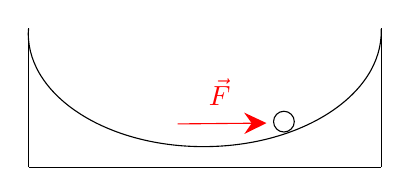
\begin{tikzpicture}[x=0.75pt,y=0.75pt,yscale=-1,xscale=1]
%uncomment if require: \path (0,300); %set diagram left start at 0, and has height of 300

%Straight Lines [id:da3398984480833569] 
\draw    (90,103) -- (90,170) ;


%Straight Lines [id:da39213437306955434] 
\draw    (260,103) -- (260,170) ;


%Straight Lines [id:da7536538469625644] 
\draw    (90,170) -- (260,170) ;


%Shape: Arc [id:dp6883804097522237] 
\draw  [draw opacity=0] (260,103) .. controls (260,103) and (259.87,104.01) .. (259.88,104.37) .. controls (260.12,134.75) and (222.24,159.67) .. (175.28,160.04) .. controls (128.31,160.41) and (90.05,136.08) .. (89.81,105.71) .. controls (89.81,105.53) and (89.81,105.35) .. (89.81,105.17) -- (174.84,105.04) -- cycle ; \draw   (259.85,103.29) .. controls (259.87,103.65) and (259.87,104.01) .. (259.88,104.37) .. controls (260.12,134.75) and (222.24,159.67) .. (175.28,160.04) .. controls (128.31,160.41) and (90.05,136.08) .. (89.81,105.71) .. controls (89.81,105.53) and (90,103) .. (90,103) ;
%Shape: Circle [id:dp54266808828771] 
\draw   (208,148) .. controls (208,145.24) and (210.24,143) .. (213,143) .. controls (215.76,143) and (218,145.24) .. (218,148) .. controls (218,150.76) and (215.76,153) .. (213,153) .. controls (210.24,153) and (208,150.76) .. (208,148) -- cycle ;
%Straight Lines [id:da8066991195909812] 
\draw [color={rgb, 255:red, 255; green, 0; blue, 0 }  ,draw opacity=1 ]   (161.8,149.1) -- (202.6,148.72) ;
\draw [shift={(204.6,148.7)}, rotate = 539.46] [fill={rgb, 255:red, 255; green, 0; blue, 0 }  ,fill opacity=1 ][line width=0.75]  [draw opacity=0] (10.72,-5.15) -- (0,0) -- (10.72,5.15) -- (7.12,0) -- cycle    ;


% Text Node
\draw (120,147) node  [align=left] {};
% Text Node
\draw (182,133.8) node [color={rgb, 255:red, 255; green, 0; blue, 0 }  ,opacity=1 ]  {$\vec{F}$};


\end{tikzpicture}

%	\centerline{\includegraphics[width=0.5\linewidth]{Figuras/Ch08/uniforme1.png}}
}

\section*{Exercícios}

\frame{
	\frametitle{Exercícios}
	\begin{block}{}

		01. Num campo elétrico uniforme de intensidade $E = \SI{5.0e3}{\newton\per\coulomb}$ direção vertical e sentido de baixo para cima, é colocada em repouso uma partícula $q = \SI{2.0}{\micro\coulomb}$. Sendo $m = \SI{4.0}{\gram}$ a massa da partícula e desprezando as ações da gravidade, determine a aceleração adquirida pela partícula.

		\vspace{0.5cm}

		02. Considere uma esfera metálica de raio $R$, com uma carga elétrica $Q$ uniformemente distribuída em sua superfície. Num ponto $P$, a uma distância $2R$ do centro da esfera, o campo elétrico vale $E$. Determine o valor do	campo elétrico a uma distância $3R$ da superfície da esfera.
	\end{block}
}


\section*{Referências}

\frame{
	\frametitle{Referências e Exercícios Complementares}
	\begin{itemize}
		\item Física, Ciência e Tecnologia – Vol 3. PENTEADO, Paulo César M; TORRES, Carlos Magno A. Ed. Moderna (2006)
	\end{itemize}
	%\centering{\alert{Página 36 - \textbf{1.6.1 até 1.6.5, 1.6.17 até 1.6.19}}} \\
	%https://www.youtube.com/watch?v=IUgS7Uw-qBI
	\centering{\alert{Lista de exercícios 08}}
}